\documentclass[12pt,a4paper]{article}
\usepackage{fontspec}
\setmainfont{Latin Modern Roman}
\setsansfont{Latin Modern Sans}
\IfFileExists{lithuanian.ldf}{\usepackage[lithuanian]{babel}}{\usepackage[provide=*]{babel}\babelprovide[main,import]{lithuanian}}
\usepackage{amsmath,amssymb,multicol,enumitem,needspace,tikz,tcolorbox}
\usepackage[left=1.6cm,right=1.6cm,top=1.5cm,bottom=1.5cm]{geometry}
\emergencystretch=3em
\setlength{\parindent}{0pt}\setlength{\parskip}{3pt}
\setlist[enumerate,1]{label=\textbf{\arabic*.},ref=\arabic*,leftmargin=*,itemsep=7pt}
\setlist[enumerate,2]{label=\alph*),leftmargin=*,itemsep=2pt}
\newcommand{\zingsnis}[1]{\tikz[baseline=(zenklas.base)]\node[draw=black!65,fill=black!7,circle,inner sep=1pt,minimum size=5mm,font=\sffamily\bfseries\footnotesize] (zenklas) {#1};}
\newcommand{\svarbu}{\tikz[baseline=(zenklas.base)]\node[circle,draw=blue!50!black,line width=0.6pt,minimum size=4.5mm,inner sep=0pt,font=\sffamily\bfseries\small,text=blue!50!black] (zenklas) {!};}
\begin{document}
\begin{center}
{\large\sffamily\bfseries KVADRATINIS DAUGIANARIS}\\[5pt]
{\small\sffamily 2 TEMA}\\[4pt]
{\LARGE\bfseries Pilnojo kvadrato išskyrimas}\\[7pt]
{\small Andrius Berniukevičius \quad\textbar\quad Vilniaus licėjus}\\[4pt]
\rule{0.72\textwidth}{0.4pt}
\end{center}
\begin{tcolorbox}[colback=black!3,colframe=black!65,boxrule=0.6pt,arc=2mm,left=2.5mm,right=2.5mm,top=1.5mm,bottom=1.5mm]
\textbf{Kaip dirbti su šia medžiaga?}

Ši medžiaga skirta aktyviam mokymuisi: naujas mintis ir faktus atrasi spręsdamas uždavinius.
\begin{enumerate}[label=\protect\zingsnis{\arabic*},leftmargin=8mm,itemsep=1pt,topsep=2pt]
\item \textbf{Pirmiausia galvok pats.} Perskaityk sąlygą, išbandyk savo idėjas pasitelkdamas pavyzdžius ir užrašyk sprendimą taip, kaip supranti. Jei užstrigai, išbandyk konkretų skaičių arba grįžk prie panašaus ankstesnio uždavinio.
\item \textbf{Tik tada pasitikrink.} Palygink savo sprendimą su pateiktuoju. Tavo būdas gali skirtis nuo pateiktojo ir vis tiek būti teisingas. Jei suklydai, išsiaiškink savo klaidą. Jei pasinaudojai pateiktu sprendimu, išnagrinėk, kodėl kiekvienas jo žingsnis teisingas. Tada užversk sprendimą ir išspręsk uždavinį iš naujo pats.
\item \textbf{Sustok prie $\star$.} Žvaigždute pažymėti uždaviniai padeda atrasti ir suprasti svarbias idėjas, kuriomis remsimės šioje ir vėlesnėse temose. Juos išsprendęs, pabandyk savais žodžiais nusakyti, ką sužinojai ir kodėl tai teisinga.
\item \textbf{Apibendrink ir pasitikrink.} Temos pabaigoje rasi svarbiausias išvadas. Pirmiausia pamėgink jas prisiminti pats, tada palygink su pateiktomis. Savikontrolės uždavinį ($\blacklozenge$) spręsk užvertęs santrauką, o po pertraukos prie jo sugrįžk.
\end{enumerate}
Siek ne vien gauti teisingą atsakymą, bet ir suprasti, \textbf{kodėl jis teisingas ir kada atrastą mintį galėsi pritaikyti}.
\end{tcolorbox}
\textbf{Temos esmė ir tikslas.} Išmoksi pertvarkyti kvadratinius reiškinius išskirdamas pilnąjį kvadratą, suprasi, kodėl šis būdas veikia, ir galėsi jį paaiškinti geometriškai bei algebriškai.

\textbf{Prieš pradėdamas:} mokėk skaičiuoti su trupmenomis, atskliausti ir taikyti sumos bei skirtumo kvadrato formules. Kvadratinio daugianario sąvoka nagrinėta 1 temoje.

\begin{enumerate}
\item Atskliauskite ir sutraukite panašiuosius narius:
\begin{multicols}{2}\begin{enumerate}
\item $(x+3)^2$; \item $(x-4)^2$; \item $(x+\frac{1}{2})^2$; \item $(x-\frac{3}{2})^2$.
\end{enumerate}\end{multicols}
Kaip iš koeficiento prie $x$ galima nustatyti skaičių skliaustuose?
\item Turite kvadratą, kurio kraštinė $x>0$, ir $14$ vienodų stačiakampių, kurių kraštinės yra $x$ ir $1$. Iš septynių stačiakampių sudėkite $x$ ilgio ir $7$ pločio juostą. Sudėkite dvi tokias juostas ir kiekvieną kraštine, kurios ilgis $x$, priglauskite prie vienos iš dviejų gretimų pradinio kvadrato kraštinių, kaip parodyta brėžinyje. Likusią tuščią kampo dalį norite užpildyti vienetiniais kvadratėliais, kad visa figūra būtų kvadratas.
\begin{center}
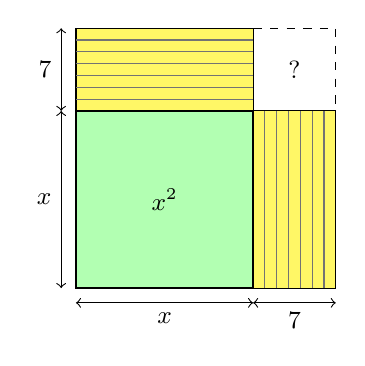
\begin{tikzpicture}[scale=0.75,every node/.style={font=\small}]
\fill[green!30] (0,0) rectangle (3,3);
\fill[yellow!60] (3,0) rectangle (4.4,3);
\fill[yellow!60] (0,3) rectangle (3,4.4);
\draw[thick] (0,0) rectangle (3,3);
\draw (3,0) rectangle (4.4,3) (0,3) rectangle (3,4.4);
\draw[dashed] (3,3) rectangle (4.4,4.4);
\foreach \i in {1,...,6}{\draw[black!55] (3+0.2*\i,0)--(3+0.2*\i,3); \draw[black!55] (0,3+0.2*\i)--(3,3+0.2*\i);}
\node at (1.5,1.5) {$x^2$}; \node at (3.7,3.7) {?};
\draw[<->] (0,-0.25)--node[below] {$x$}(3,-0.25);
\draw[<->] (3,-0.25)--node[below] {$7$}(4.4,-0.25);
\draw[<->] (-0.25,0)--node[left] {$x$}(-0.25,3);
\draw[<->] (-0.25,3)--node[left] {$7$}(-0.25,4.4);
\end{tikzpicture}
\end{center}
\begin{enumerate}
\item Kiek vienetinių kvadratėlių reikės? Paaiškinkite.
\item Užrašykite figūros plotą kaip pradinio kvadrato, stačiakampių ir mažųjų kvadratėlių plotų sumą.
\item Palyginkite šį plotą su plotu, apskaičiuotu pagal naujojo kvadrato kraštinę, ir išskirkite pilnąjį kvadratą reiškinyje $x^2+14x$.
\end{enumerate}
\item Tarkime, kad $x>0$ ir $b>0$. Kvadratas, kurio kraštinė $x$, ir du stačiakampiai, kurių kraštinės $x$ ir $\frac{b}{2}$, sudėti taip, kaip pavaizduota brėžinyje.
\begin{center}
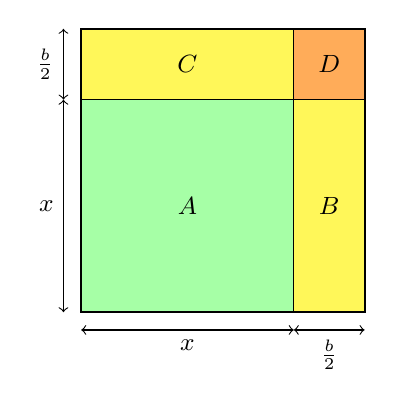
\begin{tikzpicture}[scale=0.90, every node/.style={font=\small}]
\fill[green!35] (0,0) rectangle (3,3);
\fill[yellow!65] (3,0) rectangle (4,3);
\fill[yellow!65] (0,3) rectangle (3,4);
\fill[orange!65] (3,3) rectangle (4,4);
\draw[thick] (0,0) rectangle (4,4);
\draw (3,0)--(3,4) (0,3)--(4,3);
\node at (1.5,1.5) {$A$};
\node at (3.5,1.5) {$B$};
\node at (1.5,3.5) {$C$};
\node at (3.5,3.5) {$D$};
\draw[<->] (0,-0.25)--node[below] {$x$}(3,-0.25);
\draw[<->] (3,-0.25)--node[below] {$\frac{b}{2}$}(4,-0.25);
\draw[<->] (-0.25,0)--node[left] {$x$}(-0.25,3);
\draw[<->] (-0.25,3)--node[left] {$\frac{b}{2}$}(-0.25,4);
\end{tikzpicture}
\end{center}
\begin{enumerate}
\item Apskaičiuokite $A$, $B$ ir $C$ sričių plotų sumą. Kodėl ji lygi $x^2+bx$?
\item Kokio ploto kvadrato $D$ reikia, kad būtų užpildytas didysis kvadratas? Koks yra didžiojo kvadrato kraštinės ilgis ir plotas?
\item Remdamiesi brėžiniu paaiškinkite, kodėl
\[
x^2+bx=\left(x+\frac{b}{2}\right)^2-\left(\frac{b}{2}\right)^2.
\]
\item Ar brėžinys, kuriame $\frac{b}{2}$ žymi ilgį, tiesiogiai paaiškina atvejį $b<0$? Ką reikėtų padaryti, kad lygybę galėtume pagrįsti ir šiuo atveju?
\end{enumerate}

\item $\star$ Įrodykite, kad su visomis realiosiomis $x$ ir $b$ reikšmėmis
\[
x^2+bx=\left(x+\frac{b}{2}\right)^2-\left(\frac{b}{2}\right)^2.
\]
Kodėl skliaustuose rašome $\frac{b}{2}$? Kodėl paskui atimame $\left(\frac{b}{2}\right)^2$?


\textbf{Sustok ir apibendrink.} Kaip išskirti pilnąjį kvadratą reiškinyje $x^2+bx$? Paaiškink, kodėl skliaustuose rašoma $\frac b2$ ir kodėl atimamas šio skaičiaus kvadratas.

\textbf{Pilnojo kvadrato išskyrimas} – tai reiškinio pertvarkymas taip, kad jame atsirastų kintamojo ir skaičiaus sumos arba skirtumo kvadratas. Pavyzdžiui, įrodytoje lygybėje toks kvadratas yra $\left(x+\frac{b}{2}\right)^2$. Kvadratinio daugianario užrašas $a(x-h)^2+k$, kai $a\ne 0$, o $a$, $h$ ir $k$ yra realieji skaičiai, vadinamas jo \textbf{pilnojo kvadrato pavidalu}.

\item Užrašykite reiškinius pavidalu $(x-h)^2+k$. Atsakymus patikrinkite atskliausdami.
\begin{multicols}{3}\begin{enumerate}
\item $x^2+4x$; \item $x^2+6x$; \item $x^2-8x$; \item $x^2-12x$; \item $x^2+2x$; \item $x^2-10x$; \item $x^2+14x$; \item $x^2-16x$; \item $x^2+20x$.
\end{enumerate}\end{multicols}
\item Išskirkite pilnąjį kvadratą ir patikrinkite atsakymus:
\begin{multicols}{2}\begin{enumerate}
\item $x^2+5x$; \item $x^2-3x$; \item $x^2+x$; \item $x^2-7x$; \item $x^2+\frac{3}{2}x$; \item $x^2-\frac{1}{2}x$; \item $x^2$; \item $x^2+\sqrt{2}x$.
\end{enumerate}\end{multicols}
\item Mokinys teigia: $x^2-6x=(x-3)^2-3$. Patikrinkite lygybę, paaiškinkite klaidą ir užrašykite teisingą lygybę.
\item $\star$ Tegul $a,b,x\in\mathbb R$ ir $a\ne0$.
\begin{enumerate}
\item Įrodykite, kad $ax^2+bx=a\left(x^2+\frac{b}{a}x\right)$. Kodėl skliaustuose prie $x$ yra $\frac{b}{a}$?
\item Paaiškinkite, kaip išskirti pilnąjį kvadratą reiškinyje $ax^2+bx$, pasinaudojant jau išnagrinėtu pavidalu $x^2+px$.
\item Atlikdami šiuos veiksmus išskirkite pilnąjį kvadratą reiškiniuose $2x^2-8x$ ir $-x^2+6x$. Atsakymus patikrinkite atskliausdami.
\end{enumerate}

\textbf{Sustok ir apibendrink.} Kaip išskirti pilnąjį kvadratą reiškinyje $ax^2+bx$? Į ką svarbu atkreipti dėmesį, kai $a<0$?

\needspace{8\baselineskip}
\item Užrašykite reiškinius pavidalu $a(x-h)^2+k$. Patikrinkite atskliausdami.
\begin{multicols}{2}\begin{enumerate}
\item $2x^2+8x$; \item $3x^2-12x$; \item $-x^2+6x$; \item $-2x^2-8x$; \item $2x^2+4x$; \item $-3x^2+18x$; \item $4x^2-8x$; \item $-2x^2+12x$.
\end{enumerate}\end{multicols}
\item Išskirkite pilnąjį kvadratą:
\begin{multicols}{2}\begin{enumerate}
\item $2x^2+6x$; \item $4x^2-4x$; \item $-2x^2+2x$; \item $3x^2+3x$; \item $-3x^2-6x$; \item $5x^2-5x$.
\end{enumerate}\end{multicols}
\item Mokinys užrašė $-x^2+6x=-(x-3)^2-9$.
\begin{enumerate}
\item Patikrinkite lygybę įrašydami $x=0$, tada paaiškinkite klaidą ir pataisykite lygybę.
\item Ar patikra su viena $x$ reikšme galėtų įrodyti, kad lygybė yra tapatybė? Pagrįskite pavyzdžiu.
\end{enumerate}
\item $\star$ Paaiškinkite, kaip išskirti pilnąjį kvadratą kvadratiniame daugianaryje $ax^2+bx+c$, kai jau mokate tai padaryti reiškinyje $ax^2+bx$. Pritaikykite savo būdą daugianariui $2x^2-8x+3$ ir patikrinkite atsakymą atskliausdami.

\textbf{Sustok ir apibendrink.} Kaip pasinaudoti jau išmoktu būdu, kai daugianaryje yra ir laisvasis narys $c$?

\item Išskirkite pilnąjį kvadratą ir atsakymą patikrinkite atskliausdami:
\begin{multicols}{2}\begin{enumerate}
\item $x^2+6x+5$; \item $x^2-8x+3$; \item $x^2+4x-3$; \item $x^2-10x+25$; \item $x^2+3x+1$; \item $x^2-x-2$.
\end{enumerate}\end{multicols}
\item Išskirkite pilnąjį kvadratą:
\begin{multicols}{2}\begin{enumerate}
\item $2x^2+8x+3$; \item $3x^2-12x+5$; \item $-x^2+6x-2$; \item $-2x^2-8x+1$; \item $2x^2+6x+4$; \item $4x^2-4x+7$; \item $-3x^2+6x+5$; \item $5x^2-5x+2$.
\end{enumerate}\end{multicols}
\item $\star$ Raskite realiuosius skaičius $h$ ir $k$, su kuriais lygybės teisingos su visomis realiosiomis $x$ reikšmėmis:
\begin{enumerate}
\item $x^2-8x+7=(x-h)^2+k$;
\item $-2x^2+12x-1=-2(x-h)^2+k$.
\end{enumerate}
Išskirkite pilnąjį kvadratą ir patikrinkite gautas lygybes atskliausdami. Tada atskliauskite dešiniąją pusę su nežinomaisiais $h$ ir $k$ ir, remdamiesi 1 temos 17 uždavinio išvada apie daugianarių koeficientus, pagrįskite, kad kitų sprendinių nėra.

\textbf{Sustok ir apibendrink.} Kaip pagrįsti, kad tam pačiam daugianariui surasti skaičiai $h$ ir $k$ yra vieninteliai?

\item $\star$ Apibendrinkite:
\begin{enumerate}
\item Mokinys, išskirdamas pilnąjį kvadratą, užrašė $x^2+6x+5=(x+3)^2+5-5$. Jis teigia, kad reikia atimti $5$, nes tai yra pradinio daugianario laisvasis narys. Ar šis sprendimas teisingas? Paaiškinkite ir išskirkite pilnąjį kvadratą.
\item Išskirkite pilnąjį kvadratą daugianaryje $-2x^2+12x+1$. Paaiškinkite, kodėl dauginant iš $-2$ svarbu pakeisti abiejų skliaustuose esančių narių ženklus.
\item Užrašykite gautą rezultatą pavidalu $a(x-h)^2+k$ ir nurodykite $a$, $h$ bei $k$. Patikrinkite atskliausdami.
\end{enumerate}
\end{enumerate}
\newpage
\begin{center}{\Large\bfseries Ką atradome?}\end{center}
Prieš skaitydamas pabandyk iš atminties pasakyti svarbiausias temos išvadas. Tada palygink savo mintis su šia atrama ir grįžk prie vietų, kurios kelia klausimų.

\begin{tcolorbox}[colback=blue!3,colframe=blue!40!black,boxrule=0.5pt,arc=1mm,colbacktitle=blue!8,coltitle=black,title={\svarbu\quad\bfseries Svarbiausios temos išvados}]
\textbf{1. Pavidalas $x^2+bx$.} Su visomis realiosiomis $x$ ir $b$ reikšmėmis
\[
x^2+bx=\left(x+\frac b2\right)^2-\left(\frac b2\right)^2.
\]
Į skliaustus įrašome pusę koeficiento prie $x$, o jos kvadratą atimame.

\textbf{2. Pavidalas $ax^2+bx$, kai $a\ne0$.} Pirmiausia iškeliame $a$ prieš skliaustus:
\[
ax^2+bx=a\left(x^2+\frac ba x\right).
\]
Skliaustuose išskiriame pilnąjį kvadratą, tada abu gautus narius padauginame iš $a$.

\textbf{3. Kvadratinis daugianaris $ax^2+bx+c$.} Išskiriame pilnąjį kvadratą reiškinyje $ax^2+bx$, pridedame $c$ ir sutraukiame skaičius.

\textbf{4. Pilnojo kvadrato pavidalas.} Kvadratinį daugianarį galima užrašyti $P(x)=a(x-h)^2+k$, kur $a\ne0$, o $a$, $h$, $k$ – realieji skaičiai. Šie skaičiai yra vieninteliai. Pavyzdžiui,
\[
3(x+4)^2-7=3(x-(-4))^2-7,\quad a=3,\quad h=-4,\quad k=-7.
\]
\textbf{5. Patikra.} Atskliaudę gautą užrašą ir sutraukę narius turime gauti pradinį reiškinį.
\end{tcolorbox}
\textbf{Ką verta užsirašyti savo atramose?} Pasirink svarbiausią temos išvadą ir užsirašyk: faktą, jo galiojimo sąlygas, kodėl jis teisingas, ir vieną savo pavyzdį. Išvadų taikymą pasitikrink toliau pateiktu $\blacklozenge$ pažymėtu uždaviniu.
\newpage
\begin{center}{\Large\bfseries Savikontrolė}\end{center}
Pirmiausia užversk temos atramą ir savarankiškai išspręsk uždavinį. Pasitikrink atsakymus, o jei kuri nors dalis kėlė sunkumų, grįžk prie atitinkamos išvados ir pabandyk dar kartą. Kitą dieną arba prieš pradėdamas kitą temą dar kartą išspręsk šį uždavinį nesinaudodamas santrauka.
\begin{enumerate}[resume]
\item $\blacklozenge$ Atlikite užduotis ir paaiškinkite savo sprendimus:
\begin{enumerate}
\item Išskirkite pilnąjį kvadratą daugianaryje $\frac12x^2+3x-1$.
\item Išskirkite pilnąjį kvadratą daugianaryje $-\frac12x^2+2x+3$.
\item Užrašykite $2(x+3)^2-5$ standartiniu pavidalu. Nurodykite ir $a$, $h$, $k$ pilnojo kvadrato pavidale $a(x-h)^2+k$.
\item Mokinys teigia, kad $-2(x^2-4x)=-2(x-2)^2-8$. Patikrinkite šią lygybę ir, jei reikia, pataisykite klaidą.
\end{enumerate}
\end{enumerate}
\newpage
\begin{center}{\Large\bfseries Atsakymai ir sprendimai}\end{center}
\begin{enumerate}
\item \textbf{a)} $x^2+6x+9$.

\textbf{b)} $x^2-8x+16$.

\textbf{c)} $x^2+x+\frac{1}{4}$.

\textbf{d)} $x^2-3x+\frac{9}{4}$. Kadangi $(x+t)^2=x^2+2tx+t^2$, skaičius skliaustuose yra pusė koeficiento prie $x$.
\item \textbf{a)} Sudėjus juostas prie dviejų gretimų kvadrato kraštinių, kampe lieka kvadratas, kurio kraštinė $7$. Jam užpildyti reikia $7\cdot7=49$ vienetinių kvadratėlių. Užpildžius kampą, gauto kvadrato kraštinės ilgis bus $x+7$.

\begin{center}
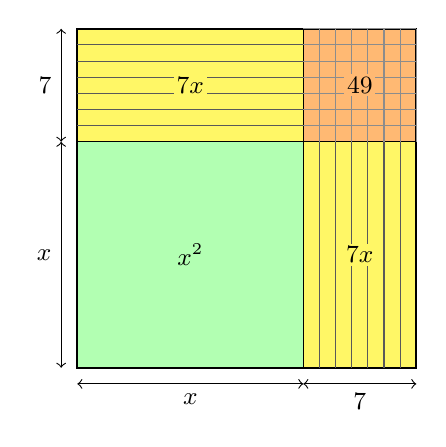
\begin{tikzpicture}[scale=0.82,every node/.style={font=\small}]
\fill[green!30] (0,0) rectangle (3.5,3.5);
\fill[yellow!60] (3.5,0) rectangle (5.25,3.5);
\fill[yellow!60] (0,3.5) rectangle (3.5,5.25);
\fill[orange!55] (3.5,3.5) rectangle (5.25,5.25);
\draw[thick] (0,0) rectangle (5.25,5.25);
\draw (3.5,0)--(3.5,5.25) (0,3.5)--(5.25,3.5);
\foreach \i in {1,...,6}{\draw[black!65] (3.5+0.25*\i,0)--(3.5+0.25*\i,3.5); \draw[black!65] (0,3.5+0.25*\i)--(3.5,3.5+0.25*\i);}
\draw[step=0.25,black!45] (3.5,3.5) grid (5.25,5.25);
\node[fill=green!30,inner sep=1pt] at (1.75,1.75) {$x^2$};
\node[fill=yellow!60,inner sep=1pt] at (4.375,1.75) {$7x$};
\node[fill=yellow!60,inner sep=1pt] at (1.75,4.375) {$7x$};
\node[fill=orange!55,inner sep=1pt] at (4.375,4.375) {$49$};
\draw[<->] (0,-0.25)--node[below] {$x$}(3.5,-0.25);
\draw[<->] (3.5,-0.25)--node[below] {$7$}(5.25,-0.25);
\draw[<->] (-0.25,0)--node[left] {$x$}(-0.25,3.5);
\draw[<->] (-0.25,3.5)--node[left] {$7$}(-0.25,5.25);
\end{tikzpicture}
\end{center}
\textbf{b)} Pradinio kvadrato plotas $x^2$, visų stačiakampių – $14x$, o pridėtų kvadratėlių – $49$. Todėl visos figūros plotas $x^2+14x+49$.

\textbf{c)} Gauto kvadrato kraštinė yra $x+7$, todėl jo plotas taip pat lygus $(x+7)^2$. Vadinasi,
\[
x^2+14x+49=(x+7)^2,\qquad
x^2+14x=(x+7)^2-49.
\]
\item \textbf{a)} Kvadrato plotas yra $x^2$, o kiekvieno iš dviejų stačiakampių – $x\cdot\frac{b}{2}=\frac{bx}{2}$. Todėl jų plotų suma yra
\[
x^2+\frac{bx}{2}+\frac{bx}{2}=x^2+bx.
\]

\textbf{b)} Trūkstamas kvadratas turi kraštinę $\frac{b}{2}$, taigi jo plotas $\left(\frac{b}{2}\right)^2$. Didžiojo kvadrato kraštinė yra $x+\frac{b}{2}$, o plotas – $\left(x+\frac{b}{2}\right)^2$.

\textbf{c)} Didžiojo kvadrato plotą sudaro sritys $A$, $B$, $C$ ir kvadratas $D$. Todėl $A$, $B$ ir $C$ sričių plotą randame iš didžiojo kvadrato ploto atimdami kvadrato $D$ plotą:
\[
x^2+bx=\left(x+\frac{b}{2}\right)^2-\left(\frac{b}{2}\right)^2.
\]

\textbf{d)} Ne: kai $b<0$, skaičius $\frac{b}{2}$ yra neigiamas, todėl negali būti atkarpos ilgis. Norėdami pagrįsti lygybę ir šiuo atveju, galime ją įrodyti algebriškai, nelaikydami $b$ ir $x$ atkarpų ilgiais. Tai padarysime kitame uždavinyje.
\item Pritaikome kvadrato formulę dešiniajai lygybės pusei ir sutraukiame narius:
\[
\left(x+\frac{b}{2}\right)^2-\left(\frac{b}{2}\right)^2
=x^2+2x\cdot\frac{b}{2}+\left(\frac{b}{2}\right)^2-\left(\frac{b}{2}\right)^2=x^2+bx.
\]
Skaičių $b$ dalijame iš $2$, nes kvadrato formulėje mišrusis narys yra $2x\cdot\frac{b}{2}=bx$. Pritaikius kvadrato formulę papildomai atsiranda $\left(\frac{b}{2}\right)^2$, todėl jį atimame: taip reiškinio reikšmė nepasikeičia.
\item \textbf{a)} $(x+2)^2-4=(x-(-2))^2-4$, todėl pavidale $(x-h)^2+k$ yra $h=-2$, $k=-4$;

\textbf{b)} $(x+3)^2-9$;

\textbf{c)} $(x-4)^2-16$;

\textbf{d)} $(x-6)^2-36$;

\textbf{e)} $(x+1)^2-1$;

\textbf{f)} $(x-5)^2-25$;

\textbf{g)} $(x+7)^2-49$;

\textbf{h)} $(x-8)^2-64$;

\textbf{i)} $(x+10)^2-100$.
\item \textbf{a)} $(x+\frac{5}{2})^2-\frac{25}{4}$;

\textbf{b)} $(x-\frac{3}{2})^2-\frac{9}{4}$;

\textbf{c)} $(x+\frac{1}{2})^2-\frac{1}{4}$;

\textbf{d)} $(x-\frac{7}{2})^2-\frac{49}{4}$;

\textbf{e)} $(x+\frac{3}{4})^2-\frac{9}{16}$;

\textbf{f)} $(x-\frac{1}{4})^2-\frac{1}{16}$;

\textbf{g)} $(x-0)^2$;

\textbf{h)} $(x+\frac{\sqrt{2}}{2})^2-\frac{1}{2}$.
\item Atskliaudę dešinę pusę gauname $(x-3)^2-3=x^2-6x+6$, todėl teiginys neteisingas. Pritaikius kvadrato formulę atsiranda $9$, tad reikia atimti būtent $9$: $x^2-6x=(x-3)^2-9$.
\item \textbf{a)} Atskliaudę gauname
\[
a\left(x^2+\frac{b}{a}x\right)=ax^2+a\cdot\frac{b}{a}x=ax^2+bx.
\]
Koeficientą $b$ dalijame iš $a$, nes atskliaudus jis vėl bus padaugintas iš $a$. Sąlyga $a\ne0$ reikalinga tam, kad galėtume dalyti iš $a$.

\textbf{b)} Iškeliame $a$ prieš skliaustus. Skliaustuose lieka anksčiau nagrinėtas pavidalas $x^2+px$, kur $p=\frac{b}{a}$. Išskiriame jo pilnąjį kvadratą, o tada padauginame abu gautus narius iš $a$.

\textbf{c)} Taikome tą patį būdą ir teigiamam, ir neigiamam koeficientui:
\[
\begin{aligned}
2x^2-8x&=2(x^2-4x)=2\bigl((x-2)^2-4\bigr)=2(x-2)^2-8;\\
-x^2+6x&=-(x^2-6x)=-\bigl((x-3)^2-9\bigr)=-(x-3)^2+9.
\end{aligned}
\]
Patikra: atskliaudę reiškinius $2(x-2)^2-8$ ir $-(x-3)^2+9$ atitinkamai gauname $2x^2-8x$ ir $-x^2+6x$.
\item \textbf{a)} $2(x+2)^2-8$;

\textbf{b)} $3(x-2)^2-12$;

\textbf{c)} $-(x-3)^2+9$;

\textbf{d)} $-2(x+2)^2+8$;

\textbf{e)} $2(x+1)^2-2$;

\textbf{f)} $-3(x-3)^2+27$;

\textbf{g)} $4(x-1)^2-4$;

\textbf{h)} $-2(x-3)^2+18$.
\item \textbf{a)} $2(x+\frac{3}{2})^2-\frac{9}{2}$;

\textbf{b)} $4(x-\frac{1}{2})^2-1$;

\textbf{c)} $-2(x-\frac{1}{2})^2+\frac{1}{2}$;

\textbf{d)} $3(x+\frac{1}{2})^2-\frac{3}{4}$;

\textbf{e)} $-3(x+1)^2+3$;

\textbf{f)} $5(x-\frac{1}{2})^2-\frac{5}{4}$.
\item \textbf{a)} Kai $x=0$, kairė pusė lygi $0$, o dešinė – $-9-9=-18$, todėl lygybė neteisinga. Klaida išryškėja atlikus pertvarkymą teisingai:
\[
-x^2+6x=-\bigl(x^2-6x\bigr)=-\bigl((x-3)^2-9\bigr)=-(x-3)^2+9.
\]
Prieš skliaustus esantis minusas pakeičia abiejų skliaustuose esančių narių ženklus.

\textbf{b)} Ne. Pavyzdžiui, lygybė $x^2=x$ teisinga, kai $x=0$, bet neteisinga, kai $x=2$, nes $4\ne2$. Viena netinkama reikšmė gali paneigti tapatybę, tačiau viena tinkama reikšmė neįrodo, kad lygybė teisinga su visomis $x$ reikšmėmis.
\item Pirmiausia išskiriame pilnąjį kvadratą pirmuosiuose dviejuose nariuose $ax^2+bx$, tada prie gauto reiškinio pridedame $c$ ir sutraukiame skaičius. Pavyzdžiui,
\[
\begin{aligned}
2x^2-8x+3&=2(x^2-4x)+3\\
&=2\bigl((x-2)^2-4\bigr)+3\\
&=2(x-2)^2-8+3\\
&=2(x-2)^2-5.
\end{aligned}
\]
Patikra: $2(x-2)^2-5=2(x^2-4x+4)-5=2x^2-8x+3$. Kiekvienas pertvarkymas išsaugo reiškinio reikšmę.
\item \textbf{a)} $(x+3)^2-4$;

\textbf{b)} $(x-4)^2-13$;

\textbf{c)} $(x+2)^2-7$;

\textbf{d)} $(x-5)^2$;

\textbf{e)} $(x+\frac{3}{2})^2-\frac{5}{4}$;

\textbf{f)} $(x-\frac{1}{2})^2-\frac{9}{4}$.
\item \textbf{a)} $2(x+2)^2-5$;

\textbf{b)} $3(x-2)^2-7$;

\textbf{c)} $-(x-3)^2+7$;

\textbf{d)} $-2(x+2)^2+9$;

\textbf{e)} $2(x+\frac{3}{2})^2-\frac{1}{2}$;

\textbf{f)} $4(x-\frac{1}{2})^2+6$;

\textbf{g)} $-3(x-1)^2+8$;

\textbf{h)} $5(x-\frac{1}{2})^2+\frac{3}{4}$.
\item \textbf{a)} Išskyrę pilnąjį kvadratą gauname $x^2-8x+7=(x-4)^2-9$. Taigi $h=4$, $k=-9$. Patikra: $(x-4)^2-9=x^2-8x+7$.

Kad pagrįstume, jog kitų porų nėra, atskliaudžiame bendrąjį užrašą: $(x-h)^2+k=x^2-2hx+h^2+k$. Pagal 1 temos 17 uždavinio išvadą apie daugianarių koeficientus gauname $-2h=-8$ ir $h^2+k=7$. Iš pirmosios lygybės $h=4$, o iš antrosios $k=7-16=-9$. Kitos poros nėra.

\textbf{b)} Išskyrę pilnąjį kvadratą gauname $-2x^2+12x-1=-2(x-3)^2+17$. Taigi $h=3$, $k=17$. Patikra: $-2(x-3)^2+17=-2x^2+12x-1$.

Bendruoju atveju $-2(x-h)^2+k=-2x^2+4hx-2h^2+k$. Prilyginę atitinkamus koeficientus gauname $4h=12$ ir $-2h^2+k=-1$. Todėl $h=3$, $k=-1+18=17$. Kitos poros nėra.
\item \textbf{a)} Sprendimas neteisingas. Atskliaudę mokinio gautos lygybės dešiniąją pusę gauname $(x+3)^2+5-5=x^2+6x+9$, o ne $x^2+6x+5$.

Kvadratui $(x+3)^2$ sudaryti reikia pridėti $9$, nes $3^2=9$; pradinio daugianario laisvasis narys yra $5$, todėl kartu atimame $9$:
\[
x^2+6x+5=x^2+6x+9-9+5=(x+3)^2-4.
\]
Patikra: $(x+3)^2-4=x^2+6x+9-4=x^2+6x+5$.

\textbf{b)} Iškeliame $-2$ prieš skliaustus, tada išskiriame pilnąjį kvadratą:
\[
\begin{aligned}
-2x^2+12x+1&=-2(x^2-6x)+1\\
&=-2\bigl((x-3)^2-9\bigr)+1\\
&=-2(x-3)^2+18+1=-2(x-3)^2+19.
\end{aligned}
\]
Dauginame abu skliaustuose esančius narius: $-2\cdot(-9)=18$. Pridėję dar $1$, gauname $k=19$.

\textbf{c)} $a=-2$, $h=3$, $k=19$. Patikra: $-2(x-3)^2+19=-2(x^2-6x+9)+19=-2x^2+12x+1$.
\item \textbf{a)} Iškeliame $\frac12$ prieš skliaustus, tada juose išskiriame pilnąjį kvadratą:
\[
\begin{aligned}
\frac12x^2+3x-1&=\frac12(x^2+6x)-1\\
&=\frac12\bigl((x+3)^2-9\bigr)-1\\
&=\frac12(x+3)^2-\frac92-1
=\frac12(x+3)^2-\frac{11}{2}.
\end{aligned}
\]
Patikra: $\frac12(x+3)^2-\frac{11}{2}=\frac12x^2+3x+\frac92-\frac{11}{2}=\frac12x^2+3x-1$.

\textbf{b)} Iškeliame neigiamą koeficientą ir dauginame iš jo abu skliaustų narius:
\[
\begin{aligned}
-\frac12x^2+2x+3&=-\frac12(x^2-4x)+3\\
&=-\frac12\bigl((x-2)^2-4\bigr)+3\\
&=-\frac12(x-2)^2+2+3=-\frac12(x-2)^2+5.
\end{aligned}
\]
Patikra: $-\frac12(x-2)^2+5=-\frac12x^2+2x-2+5=-\frac12x^2+2x+3$.

\textbf{c)} Atskliaudžiame ir sutraukiame panašiuosius narius:
\[
2(x+3)^2-5=2(x^2+6x+9)-5=2x^2+12x+13.
\]
Kadangi $x+3=x-(-3)$, tai pilnojo kvadrato pavidale $a=2$, $h=-3$, $k=-5$.

\textbf{d)} Lygybė neteisinga: kai $x=0$, jos kairė pusė lygi $0$, o dešinė – $-2\cdot4-8=-16$. Mokinys netinkamai padaugino neigiamą narį iš $-2$. Teisingai:
\[
-2(x^2-4x)=-2\bigl((x-2)^2-4\bigr)=-2(x-2)^2+8,
\]
nes $-2\cdot(-4)=8$.
\end{enumerate}
\end{document}
